\documentclass[catalan, a4paper, nobib]{tufte-handout}

% encoding
\usepackage[utf8]{inputenc}
\usepackage[T1]{fontenc}
\usepackage{lmodern}
\usepackage{babel}

\frenchspacing
\usepackage[style=spanish]{csquotes}
\MakeAutoQuote{«}{»}

\usepackage{booktabs}
\usepackage{circuitikz}
\usepackage{siunitx}
\usepackage{amsmath}
\usepackage{nicefrac}

\graphicspath{
    {fotos/}
}

% hyperlink setup / metadata
\usepackage{hyperref}
\AfterPreamble{\hypersetup{
  %%pdfauthor={},
  %%pdftitle={},
  %%pdfsubject={},
}}

% document metadata
\author{Víctor Méndez}
\title{ICOM: Pràctica 4}
\date{8-5-2024}

\begin{document}

\maketitle

\newthought{Activitat 4.1}

Generem un senyal al LaVICAD amb les següents especificacions.

\begin{figure*}[!h]
    \begin{center}
        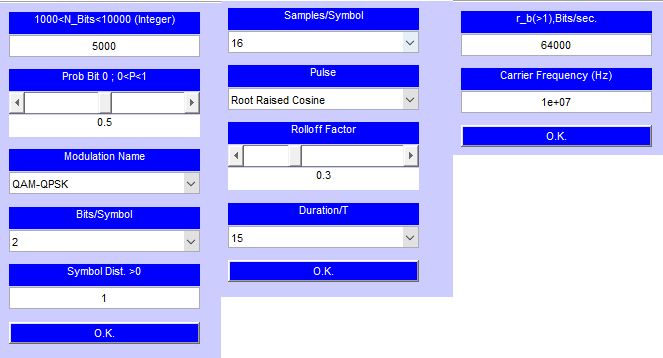
\includegraphics[width=450px]{p1.png}
    \end{center}
    \caption{Parametres escollits en base a l'estudi previ}
\end{figure*}

\newthought{Activitat 4.2}

En carregar el senyal i fer un promig de \num{50} mostres s'observa l'espectre de la figura \ref{fig:SPECTRUM}. Per acostar-nos al valor teòric de l'amplada de banda configurem l'OBW per que consideri el \num{99.6}\% de la potència (veure figura \ref{fig:OBW}). L'amplada mesurada es de \qty{41.56}{\kilo\hertz}.

\begin{figure*}
    \begin{center}
        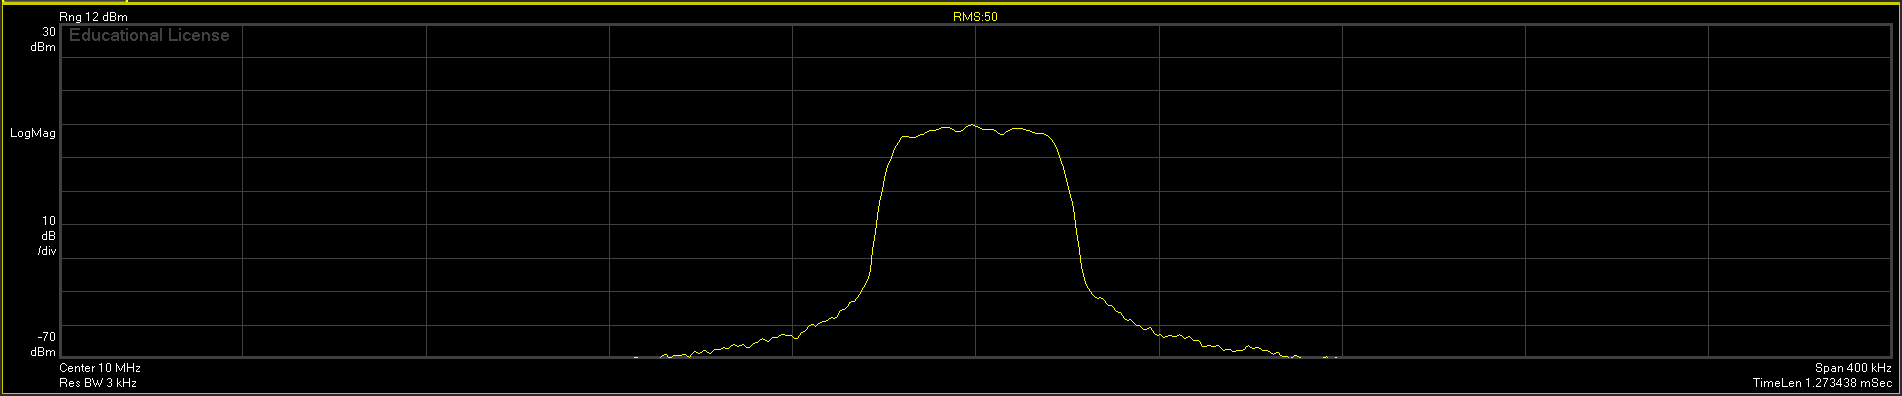
\includegraphics[width=450px]{p2_1.png}
    \end{center}
    \caption{Espectre promig del senyal}
    \label{fig:SPECTRUM}
\end{figure*}

\begin{figure*}
    \begin{center}
        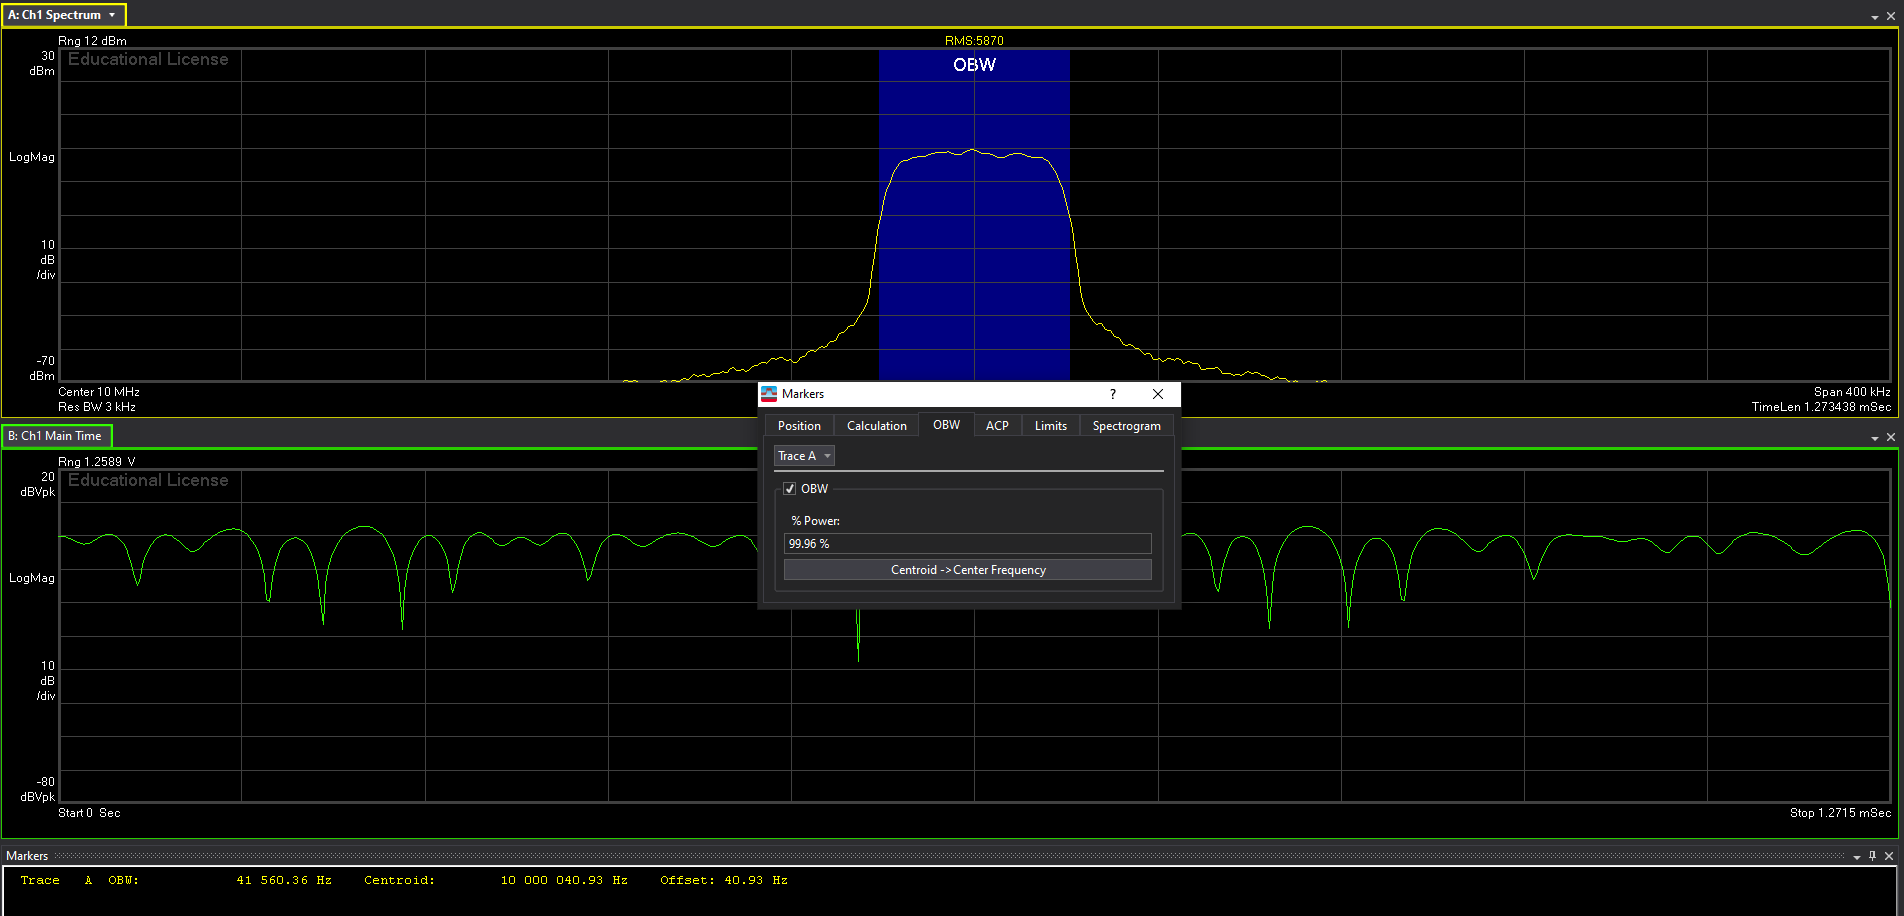
\includegraphics[width=445px]{p2_2.png}
    \end{center}
    \caption{Us del OBW}
    \label{fig:OBW}
\end{figure*}

\newthought{Activitat 4.3}

El format utilitzat és QPSK amb un Symbol Rate de \qty{32}{\kilo\hertz} i un filtre Root Raised Cosine de Alpha \num{0.3}.

\begin{figure}[!h]
    \begin{center}
        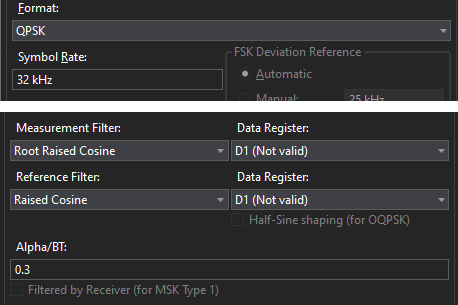
\includegraphics[width=285px]{p3.png}
    \end{center}
    \caption{Configuració proposada per a la decodificació del senyal}
\end{figure}

\newpage

\newthought{Activitat 4.4}

A recepció no hi ha cap problema de sincronisme i el filtre d'adaptació és idèntic al pols conformador. La apertura del diagrama d'ull en aquestes condicions val $\frac{d}{D}=\num{1}$.

\begin{figure}[!h]
    \begin{center}
        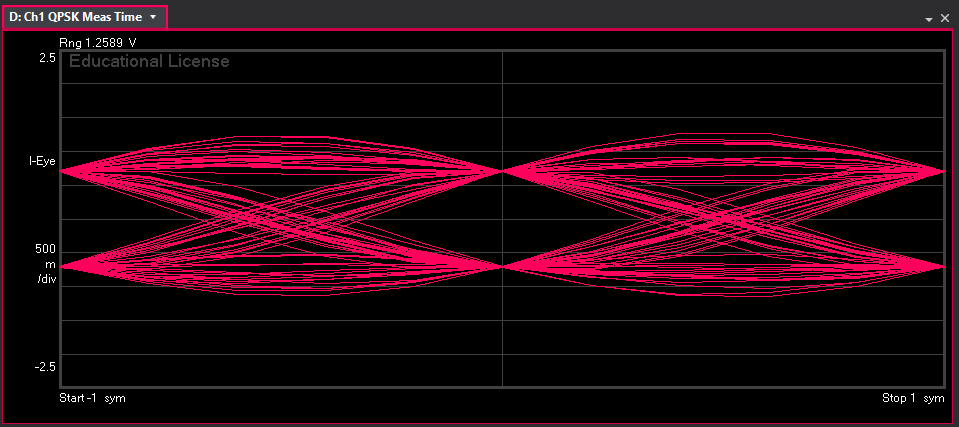
\includegraphics[width=285px]{p4.png}
    \end{center}
    \caption{Diagrama d'ull de la part en fase del senyal}
\end{figure}

\newpage

\newthought{Activitat 4.5}

La apertura del diagrama ara val $\frac{d}{D}=\frac{\num{0.64}}{\num{0.77}}=\num{0.83}$. El filtre d'adaptació ja no és idèntic al conformador, la recepció ja no és perfecta i per tant empitjora la apertura del diagrama d'ull.

El procediment seguit per fer les mesures consisteix a posar un marker a la visualització del component en fase en format real enllaçat amb el format d'ull i moure'l fins a aconseguir un marker en la posició desitjada (figura \ref{fig:MARKER}). Hi haurà distorsió màxima quan hi hagi un canvi de símbol després d'haver enviat el mateix símbol molts cops.

\begin{figure}[!h]
    \begin{center}
        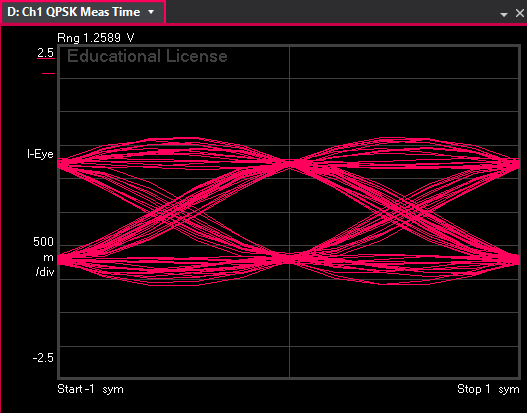
\includegraphics[width=290px]{p5.png}
    \end{center}
    \caption{Diagrama d'ull en condicions no ideals; filtre d'adaptació mal configurat}
\end{figure}

\begin{figure}
    \begin{center}
        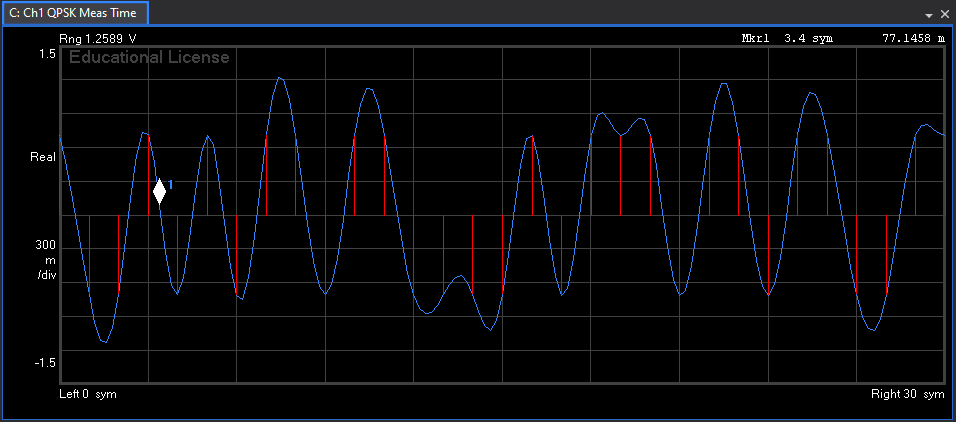
\includegraphics[width=290px]{p5_2.png}
    \end{center}
    \caption{Component en fase en format real}
    \label{fig:MARKER}
\end{figure}

\newpage

\newthought{Activitat 4.6}

Generem i carreguem un senyal QPSK com el que s'ha fet servir fins ara però amb soroll gaussià additiu de $\nicefrac{E_b}{N_0}=\qty{15}{\deci\bel}$. El soroll provoca una apertura encara pitjor a la que s'ha vist a l'apartat anterior; $\frac{d}{D}=\frac{\num{0.57}}{\num{0.90}}=\num{0.64}.$

Per obtenir les mesures es fa servir el mateix procediment descrit a l'apartat anterior.

\begin{figure}
    \begin{center}
        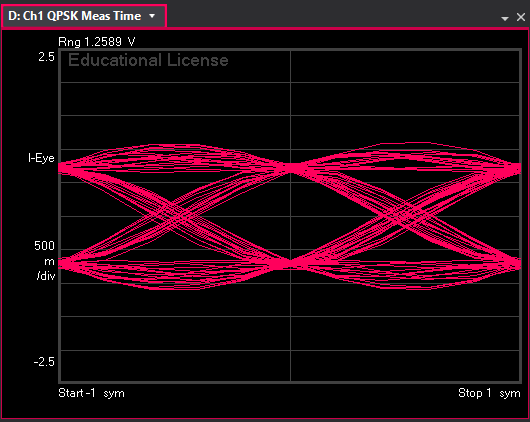
\includegraphics[width=290px]{p6.png}
    \end{center}
    \caption{Diagrama d'ull amb soroll gaussià}
\end{figure}

\end{document}